\section{Lektion 01-03-2018}

\begin{enumerate}
	\item Impulsrepsonser
	\item Auralisation af rum
	\item Binaural Analysis
\end{enumerate}

\noindent\fbox{\parbox{\textwidth}{
\begin{itemize}
	\item \textbf{Pensum:} 
	\begin{enumerate}
		\item Master Handbook of Acoustics, ch. 26 (5. edition) or \\ch. 30 (6. edition)
		\item Modelling Acoustic Spaces For Audio Virtal Reality, \\U. Peter Svensson
	\end{enumerate}
	\item \textbf{Opgaver:} 
	\begin{enumerate}
		\item Lyd og Akustik - Lektion 6 - opgaver og øvelser
	\end{enumerate}
\end{itemize}
}} \vspace{3mm}


\subsection{Impulsrepsonser}
\begin{itemize}
	\item Image Source Method og Ray Tracing kan bruges til at bestemme RIR (Room Impulse Response).
	\item Medregner frekvensafhængige karakteristikker såsom absorptionskoefficienter for materialer og højtalerens impulsrespons.
\end{itemize}
\newpage

\subsection{Auralisation af rum}
\begin{itemize}
	\item Beregning af RIR (Room Impulse Response) og derefter BRIR (Binaural Room Impulse Response) er nødvendigt.
	\item Disse impulsresponser foldes med et signal som enten skal være syntetisk genereret eller optaget i lyddødt rum (tørt signal). 
\end{itemize}

\begin{figure} [H]
	\centering
	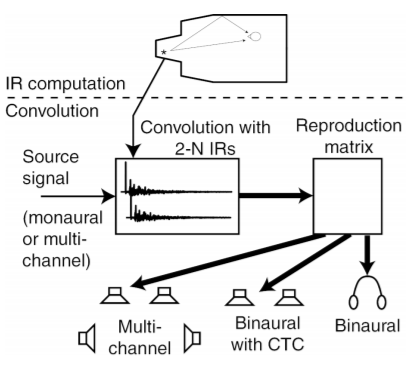
\includegraphics[width=.6\linewidth]{graphics/21.png}
	\caption{Auralisation system med impulsresponse (IR) og foldning.}
	\label{fig:21}
\end{figure}

\subsection{Binaural Analysis}
\begin{itemize}
	\item Lytteren bliver karakteriseret med overførelsesfunktion HTRF (head-related transfer function).
	\item Differensen i responset ved hvert øre, med og uden en lytter tilstede.
	\item Information om arrival time, energi, og dets vinkel i forhold til receiveren (venstre/højre øre).
	\item Retningsopfattelse er vanskelig når ITD er nul ( < \SI{10}{\micro\second}).
	\item Eneste hjælp er det ydre øres	frekvensfarvning.
	\item Vi benytter små hoveddrejninger for at forbedre lokalisationen.
\end{itemize}

\newpage
\begin{itemize}
	\item Head-Related Transfer Function (HRTF)
\end{itemize}

\begin{figure} [H]
	\centering
	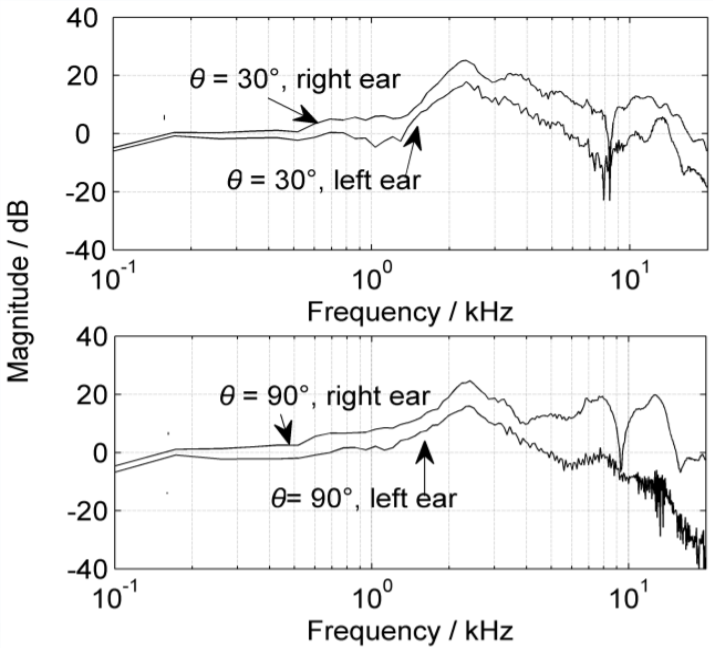
\includegraphics[width=.7\linewidth]{graphics/48.png}
	\caption{Head-Related Transfer Function (HRTF).}
	\label{fig:48}
\end{figure}

\begin{itemize}
	\item Interaural Time Difference (ITD) 
	\item Interaural Level Difference (ILD)
\end{itemize}


\begin{figure} [H]
	\centering
	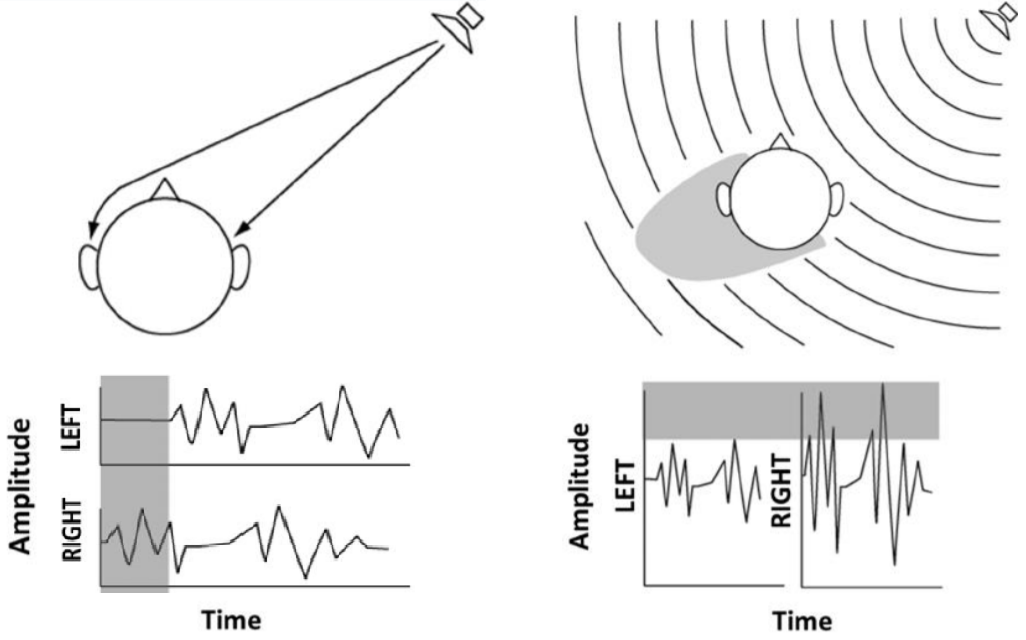
\includegraphics[width=.7\linewidth]{graphics/47.png}
	\caption{V: ITD. H: ILD.}
	\label{fig:47}
\end{figure}
\newpage
\begin{itemize}
	\item Precedence effekt
	\begin{itemize}
		\item \textit{Haas effect – Law of the first wave front}.
		\item Fantomkilder ved stereo.
	\end{itemize}
\end{itemize}

\begin{figure} [H]
	\centering
	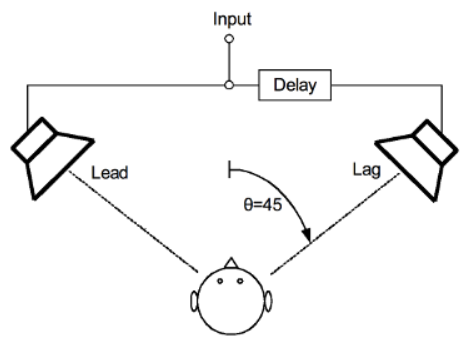
\includegraphics[width=.6\linewidth]{graphics/49.png}
	\caption{Haas effekt.}
	\label{fig:49}
\end{figure}

\begin{itemize}
	\item Ekko kan være op til \SI{10}{\decibel} kraftigere end den direkte lyd uden at ændre retningsopfattelse.
\end{itemize}